In this chapter we wish to introduce different methods to test hypotheses, where the primary focus will be t-statistics, F-statistics and coefficient of determination. 
With these tests we wish to determine the reliability of out linear regression model when it has been used on real data.
As an addition to the Gauss-Markov assumptions from chapter \ref{ch:Multip_linear_regresssion}, we will take a step further with the following assumption that imposes an additional restriction on the errors. 

\begin{assumption}[Normality of Errors] \label{as:normality_of_errors}
    Conditional on $\mathbf{X}$, the $\varepsilon_i$ are independent and identically distributed as $N(0, \sigma^2)$. Equivalently, $\boldsymbol{\varepsilon}$ given $\mathbf{X}$ is distributed as multivariate normal with mean zero and variance-covariance matrix $\sigma^2 \mathbf{I}_{n \times n}$, i.e. $\boldsymbol{\varepsilon} \sim N_n(\mathbf{0}, \sigma^2 \mathbf{I}_{n \times n})$.
\end{assumption}

\section{The t-test}
One way to test hypothesis about any single parameters in the true regression function is to make use of the t-test. 
A t-test is an inferential statistic determining whether or not the difference between two t statistics, e.g. the means of two groups, is significant. First we need a definition.

\begin{definition}
    Let $Z \sim N(0,1)$ 
\end{definition}

Recall that OLS produces unbiased estimates c.f. theorem \ref{th:unbiasedness_of_ols}, let $d_j=(\textbf{X}^\top\textbf{X})^{-1}_{jj}$ denote the $j$'th diagonal element of $(\textbf{X}^\top \textbf{X})^{-1}$, let $\hat{\beta}_j(\textbf{y})$ denote the $j$'th coordinate of the MLE $\hat{\beta}(\textbf{y})$ and $\hat{\sigma}^2(\textbf{y})$ denote the usual estimate for $\sigma^2$ as in \eqref{eq:sigma_hat_2_n-k-1}.

In order to construct a hypothesis test, the following result is needed.

\begin{theorem} [Test of Individual Parameters] \label{th:t_distribution}
Let $\beta_{0j}$ be given and consider the hypothesis $\mathcal{H}_0 \ : \ \hat{\beta}_j=\beta_{0j}$. Under the assumptions \ref{as:linear_in_the_parameters}, \ref{as:no_perfect_collinearity}, \ref{as:zero_conditional_mean}, \ref{as:homoskedasticity_and_no_serial_correlation} and \ref{as:normality_of_errors} the t-test for $\mathcal{H}_0$ is given by
\begin{align}\label{eq:t-test}
   t_j(\textbf{y};\beta_{0j}) = \frac{\hat{\beta}_j - \beta_{0j}}{\sqrt{d_j\hat{\sigma}^2(\textbf{y})}}\sim t_{n-k-1}, \quad \text{for} \ j=1,\ldots,k
\end{align}
where $k+1$ is the number of unknown parameters in the population model \eqref{eq:multiple_linear_regression}, $n-k-1$ is the degrees of freedom and large values of $|t_j(\textbf{y};\beta_{0j})|$ are critical for $\mathcal{H}_0$.

The p-value is
\begin{align}
    p(\textbf{y},\beta_{0j})=P\Big(|t_j(\textbf{Y};\beta_{0j})|\geq |t_j(\textbf{y};\beta_{0j})|\Big).
\end{align}
The p-value is the probability that, if the null hypothesis were true, sampling variation would produce an estimate that is further away from the hypothesised parameter value than our data estimates.  
Thus it would lie in the tails of the pdf of the t-distribution seen in figure \ref{fig:t_distribution}.
Meaning that a low p-value is evidence against $\mathcal{H}_0$.

Furthermore, for $0<\alpha<1$, using the t-test at level $\alpha$, the limits of a ($1-\alpha$)-confidence interval for $\beta_j$ is
\begin{align} \label{eq:t_statistic}
    \hat{\beta}_{j}(\textbf{y}) \pm t_{1-\alpha/2}(n-k-1)\sqrt{d_j\hat{\sigma}^2(\textbf{y})}
\end{align}
which corresponds to those cases where we accept the hypothesis that $\beta_j$ takes a specific value.
\end{theorem}
\begin{proof}
Recall due to the assumptions \ref{as:linear_in_the_parameters}, \ref{as:no_perfect_collinearity}, \ref{as:zero_conditional_mean}, \ref{as:homoskedasticity_and_no_serial_correlation} and \ref{as:normality_of_errors} example \ref{ex:MLE_for_model} showed that

\begin{align} \label{eq:th_t_test}
    \hat{\betabold}(\textbf{Y}) \sim N_k(\betabold,\sigma^2(\textbf{X}^T\textbf{X})^{-1})
\end{align}
which entails
\begin{align*}
    &\hat{\beta}_j(\textbf{Y})\sim N(\beta_j , \sigma^2d_j) \\
    \Leftrightarrow &  (\hat{\beta}_j(\textbf{Y})-\beta_j) \sim N(0,\sigma^2d_j)
\end{align*}
and so
\begin{align*}
    (\hat{\beta}_j(\textbf{Y})-\beta_j)/\sqrt{d_j\sigma^2(\textbf{Y})} \sim N(0,1) \quad \text{and} \quad \hat{\sigma}^2(\textbf{Y}) \sim \sigma^2\chi^2 (n-k-1)/(n-k-1)
\end{align*}
are independent.
The distribution of $\hat{\sigma}^2$ comes from \eqref{eq:sigma_hat_2_n-k-1}, so
\begin{align*}
    \hat{\sigma}^2(\textbf{y}) = \dfrac{1}{(n-k-1)}\sum_{i=1}^n \hat{\varepsilon}_i^2
\end{align*}
which is a sum of squared independent normally distributed random variables and therefore
\begin{align*}
\hat{\sigma}^2(\textbf{Y}) \sim \sigma^2 \chi^2(n-k-1)/(n-k-1).    
\end{align*}
Hence
\begin{align*}
    t_j(\textbf{Y};\beta_j)=\frac{(\hat{\beta}(\textbf{Y})-\beta_j)/\sqrt{d_j\sigma^2(\textbf{Y})}}{\sqrt{d_j\hat{\sigma}^2(\textbf{Y})/d_j\sigma^2}} \sim t(n-k-1)
\end{align*}
and the first part of the theorem composed of \eqref{eq:th_t_test} is verified, and second part follows immediately. 
\end{proof}

The pdf of the t distribution has a shape that is similar to the standard normal distribution. Except that it is more spread out in the tails and thus has larger areas in the tails. In figure \ref{fig:t_distribution} the pdf of the t distribution is plotted for various degrees of freedom compared to the standard normal distribution. 

\begin{figure}[H]
    \centering
    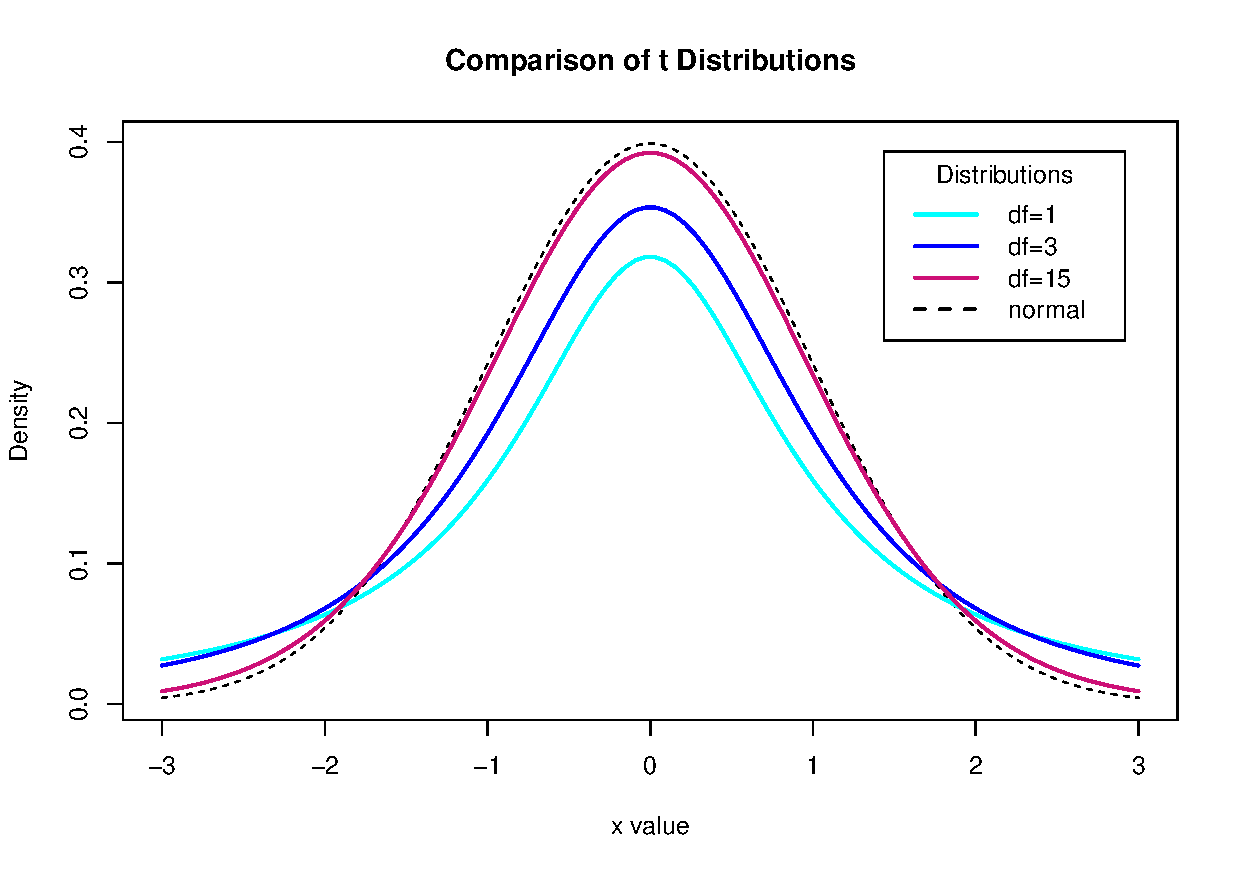
\includegraphics[width = 0.8\textwidth]{figures/t_distribution.pdf}
    \caption{The t distribution for various DF compared to the standard normal distribution.}
    \label{fig:t_distribution}
\end{figure}

Clearly, as the degrees of freedom increases, the t distribution approaches the standard normal distribution, so $t_n \rightarrow N(0,1)$ for $n\rightarrow \infty$. This also follows from the Central Limit Theorem, presented later in this chapter in theorem \ref{th:Central_limit_theorem}. 

In the case of testing OLS estimates, we test if the estimates are anything other than zero. In this case, we test against the two-tailed alternatives and therefore the primary interest is testing the null hypothesis
\begin{align} \label{eq:t_test_h0}
    \mathcal{H}_0:\beta_j=0.
\end{align}
In this case the alternative hypothesis is
\begin{align} \label{eq:t_test_ha}
    \mathcal{H}_1 : \beta_j \neq 0,
\end{align}
which means, that $\textbf{x}_j$'s effect on the expected value $\textbf{y}$ can be both positive or negative.
Since after controlling for all other independent variables than $\textbf{x}_j$, $\beta_j$ measures the partial effect of $\textbf{x}_j$ on the expected value of $\textbf{y}$. 
Thus \eqref{eq:t_test_h0} means that, after $\textbf{x}_1,\textbf{x}_2, \ldots, \textbf{x}_{j-1}, \textbf{x}_{j+1}, \ldots, \textbf{x}_k$ have been accounted for, $\textbf{x}_j$ has no effect on the expected value for $\textbf{y}$ since $\beta_j=0$. 
For $\textbf{x}_j$ having a partial effect on the expected value of $\textbf{y}$, the value of $\beta_j$ has to be anything other than zero.

In practice, $\hat{\beta}_j$ will not be zero, whether or not $\mathcal{H}_0$ is true.
Therefore the question is rather how to determine how far $\hat{\beta}_j$ is from zero. 
The further the sample value of $\hat{\beta}_j$ is from zero, the bigger is the evidence against $\mathcal{H}_0$. 
However, the larger the standard error is of $\hat{\beta}_j$, the smaller is the evidence against $\mathcal{H}_0$. 
Thus $t_{\hat{\beta}_j}$ is a ratio of how many estimated standard deviations $\hat{\beta}_j$ is away from zero.
In general the larger value of $t_{\hat{\beta}_j}$, the larger the evidence against $\mathcal{H}_0$. 
The precise rule for rejecting $\mathcal{H}_0$ depends on the alternative hypothesis and the chosen significance level.
The t value in \eqref{eq:t_statistic} is found using the inverse of the CDF of the t distribution with $(n - k - 1)$ degrees of freedom evaluated in $(1-\alpha/2)$. 
Since the t distribution is symmetric, $\pm t_{1-\alpha/2}$ is the same as $\mp t_{\alpha/2}$.

\begin{example} [Testing Against Two-tailed Alternative Hypothesis] \label{ex:ttest}
We use the dataset CARS in Rstudio to estimate a model explaining the distance taken to stop given the speed of the car.
The test is two-tailed, therefore we test the null hypothesis $\mathcal{H}_0:\beta_1=0.$
We complete the t-test at level $\alpha=0.05$ which gives the limits of a 95\%-confidence interval for $\hat{\beta}_j$.
We obtain the estimated model
\begin{align*}
    \textbf{y}_{dist} = \hat{\boldsymbol{\beta}} \boldsymbol{X}_{speed},
\end{align*}
with values listed in the following table.

\begin{table}[H]
\centering
\begin{tabular}{lrrrr}
\toprule
\textbf{term} & \textbf{estimate} & \textbf{std.error} & \textbf{t value} & \textbf{p.value}\\
\midrule
(Intercept) & -17.579095 & 6.7584402 & -2.601058 & 0.0123188\\
speed & 3.932409 & 0.4155128 & 9.463990 & 0.0000000\\
\bottomrule
\end{tabular}
\end{table}
The value of the parameter $\hat{\beta}_1=3.932409$ with t value $t_1(\hat{\beta}_1) = 9.464$ which is significant because of the low p value. 
Therefore we reject the null hypothesis at the 5\% level. This is illustrated in figure \ref{fig:t_distributionplot1}, where the dotted lines illustrates the respective end and beginning of the the rejection regions and the red line represents the value of our estimate. 
In the figure it is clear, that we are far into the tail of the null distribution which also indicates a small p value. 
This indicates, that our observed $\hat{\beta}_1$ is more extreme than what is reasonably expected if the null hypothesis were true.
\begin{figure}[H]
    \centering
    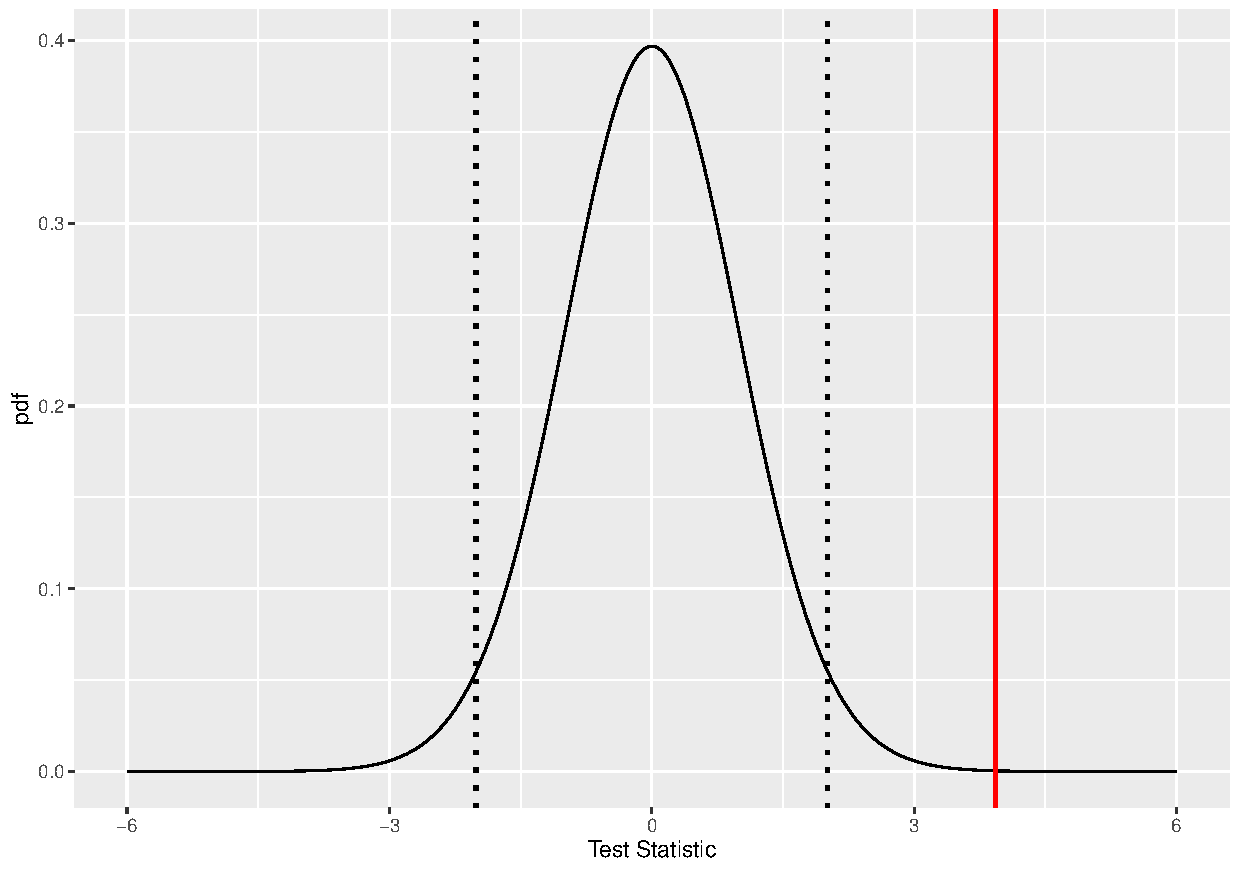
\includegraphics[width = 0.7\textwidth]{figures/Nanna/t_distributionPlot.pdf}
    \caption{5 \% rejection rule for $\mathcal{H}_a:\beta_1\neq0$ with 48 degrees of freedom and the observed value $\hat{\beta}_1=3.932409$.}
    \label{fig:t_distributionplot1}
\end{figure}
The t value is found by the inverse of the CDF where we obtain the t values of chosen probabilities. 
The $95\%$-significance level, means that we evaluate the inverse of the CDF in $0.025$ and $0.975$. 
This is illustrated in figure \ref{fig:CDF_inverse} where the intersection of the dotted lines gives the t values.
\begin{figure}[H]
    \centering
    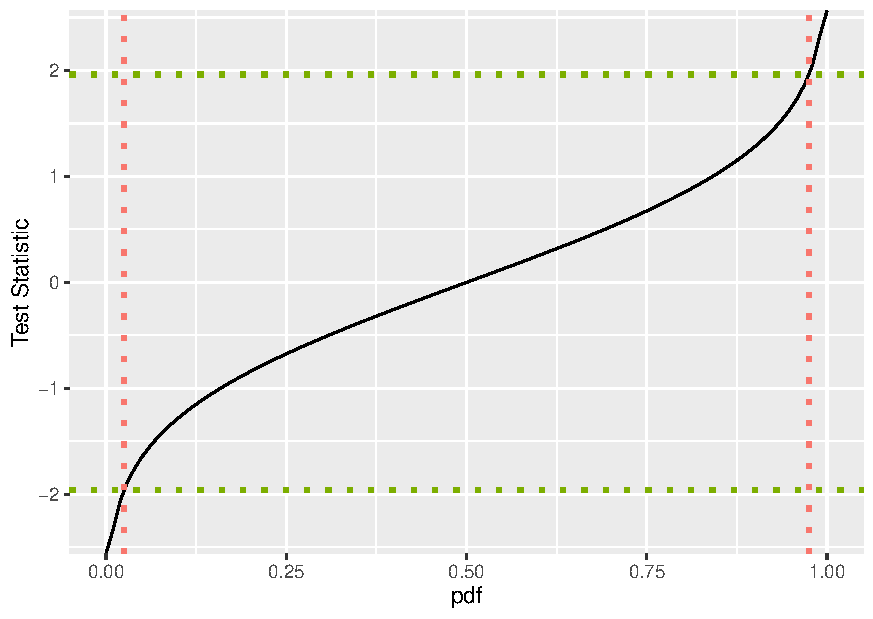
\includegraphics[width = 0.7\textwidth]{figures/Nanna/CDF_inverse.pdf}
    \caption{The inverse of the CDF in which we obtain the t value for $\mathcal{H}_0$ of the chosen $95\%$-significance level.}
    \label{fig:CDF_inverse}
\end{figure}
Now we have concluded, that speed has a statistically significant effect on the distance at a 95\%-confidence level. 
By computing the limits of a 95\%-confidence interval for $\hat{\beta}_1$ (speed), we find the 95\%-confidence interval which we expect contains the ``true'' parameter.
The 95\%-confidence intervals for $\hat{\beta}_1$ is listed in the following table.
\begin{table}[H]
\centering
\begin{tabular}{lrr}
\toprule
 & \textbf{2.5 \%} & \textbf{97.5 \%}\\
\midrule
(Intercept) & -31.167850 & -3.990340\\
speed & 3.096964 & 4.767853\\
\bottomrule
\end{tabular}
\end{table}
Note that the confidence interval for the parameter speed does not contain 0, as expected.
From this lower and upper bound of the confidence intervals of the parameters, we can plot the area in which we expect the ``true'' line to be. 
In figure \ref{fig:t_distributionplot2} the blue line is our estimated model and the shaded area is the 95\%-confidence interval of the model. 
\begin{figure}[H]
    \centering
    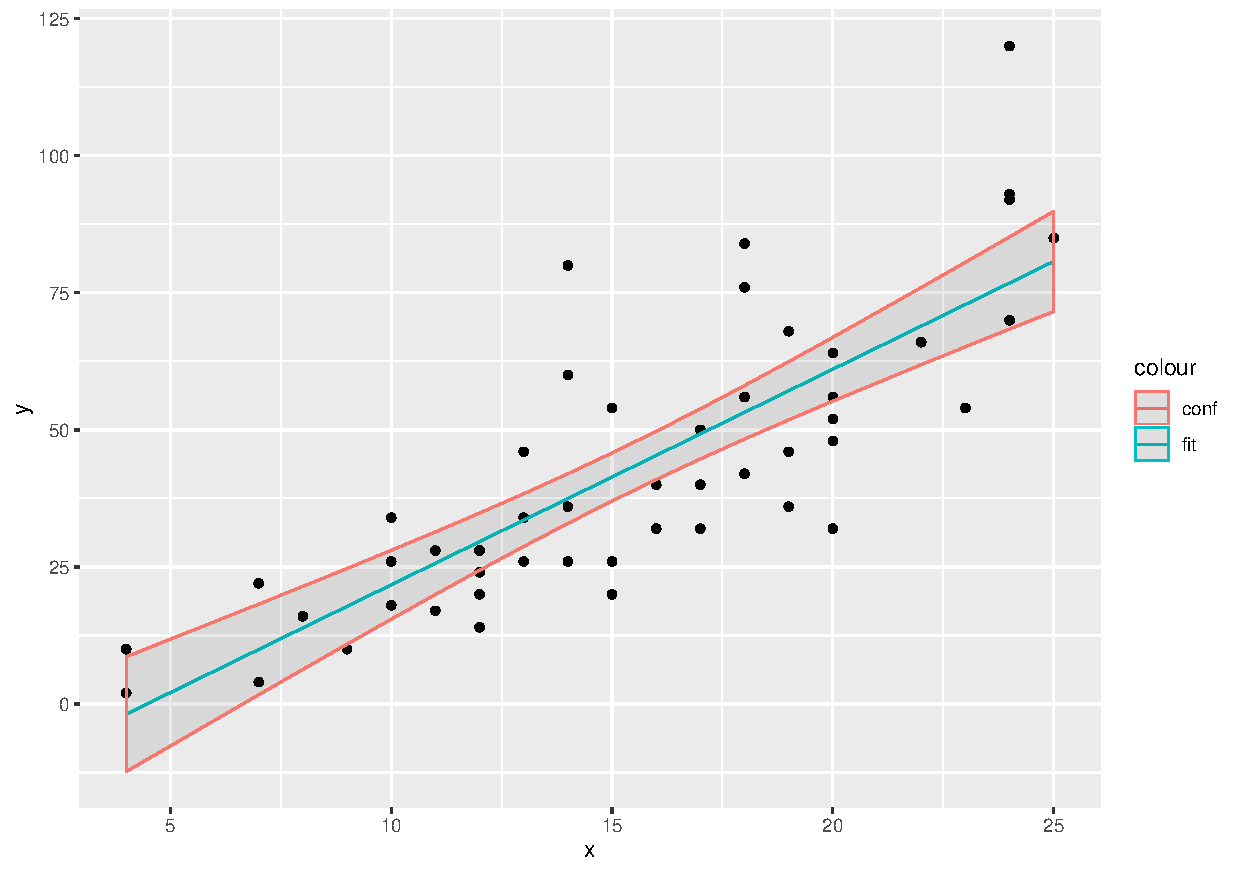
\includegraphics[width = 0.7\textwidth]{figures/Nanna/Konfidensinterval.pdf}
    \caption{Plot of the observed values, the fitted regression line and its $95\%$-confidence intervals in which we expect the ``true'' line to be.}
    \label{fig:t_distributionplot2}
\end{figure}
\end{example}

\section{Prediction}
It is often wanted to deduce information about future observations based on the existing fitted regression model. 
Due to this, prediction intervals are introduced as an estimate of an interval that contains a future observation with a certain probability with respect to already observed data.

In this section we assume a general linear model $\textbf{Y}\sim N_n(\textbf{X}\beta, \sigma^2 I_n)$, where the design matrix $\textbf{X}$ has full rank $(k+1)<n$, and where $\betabold \in \mathbb{R}^{(k+1)}$ and $\sigma^2>0$ are unknown. Suppose an observed realization of $\textbf{Y}=\textbf{y}$, however, the future random variable $\textbf{Y}_{n+1}$, where
\begin{align*}
    Y_{n+1}\sim N(\textbf{x}^\top_{n+1}\betabold,\sigma^2)
\end{align*}
are independent of $\textbf{Y}$ and where $\textbf{X}$ and $\textbf{x}_{n+1}\in\mathbb{R}^{(k+1)}$ are known. 
The natural prediction value for $\textbf{Y}_{n+1}$ is the MLE for its mean, that is c.f. \eqref{eq:betahat_y}
\begin{align*}
    \hat{Y}_{n+1}(\textbf{y})=\textbf{x}^\top_{n+1}\hat{\betabold}(\textbf{y}).
\end{align*}
The corresponding random variable $\hat{Y}_{n+1}(\textbf{Y})$ is called the predictor for $Y_{n+1}$. 
We now want to determine the variability of $Y_{n+1}$.

Given that $\hat{\betabold} \sim N_k(\betabold,\sigma^2(\textbf{X}^\top\textbf{X})^{-1})$ then $\hat{Y}_{n+1}(\textbf{Y})\sim N(\textbf{x}^\top_{n+1}\betabold,\sigma^2\textbf{x}^\top_{n+1}(\textbf{X}^\top\textbf{X})^{-1}\textbf{x}_{n+1})$ and $Y_{n+1}\sim N(\textbf{x}^\top_{n+1}\betabold,\sigma^2)$ are independent. Thus we obtain uncertainty of the estimate
\begin{align*}
    Y_{n+1}-\hat{Y}_{n+1} \sim N(0, \sigma^2(1+\textbf{x}^\top_{n+1}(\textbf{X}^\top\textbf{X})^{-1})).
\end{align*}

Further the variance estimator
\begin{align*}
    \hat{\sigma}^2(\textbf{Y})=\frac{\|\textbf{Y} - \textbf{X}( \textbf{X}^\top\textbf{X} )^{-1}\textbf{X}^\top\textbf{Y}\|^2}{n-(k+1)} \sim \frac{\chi^2(n-(k+1))}{(n-(k+1))}
\end{align*}
is independent of $Y_{n+1}-\hat{Y}_{n+1}(\textbf{Y})$ because of independence of data. Since $\hat{\sigma}^2(\textbf{Y})$ is independent of $\hat{\betabold}(\textbf{Y})$ then $\hat{\sigma}^2(\textbf{Y})$ is also independent of $Y_{n+1}-\hat{Y}_{n+1}$. From this we define
\begin{align*}
    T=\frac{Y_{n+1}-\hat{Y}_{n+1}(\textbf{Y})}{\sqrt{\hat{\sigma}^2(\textbf{Y})(1+\textbf{x}^\top_{n+1}(\textbf{X}^\top\textbf{X})^{-1}\textbf{x}_{n+1})}}
\end{align*}
and recall the proof of theorem \ref{th:t_distribution} from which we conclude that
\begin{align*}
    T=\frac{Y_{n+1}-\hat{Y}_{n+1}(\textbf{Y})/\sqrt{\sigma^2(1+\textbf{x}^\top_{n+1}(\textbf{X}^\top\textbf{X})^{-1}\textbf{x}_{n+1})}}{\sqrt{\hat{\sigma}^2(\textbf{Y})/\sigma^2}} \sim t(n-(k+1)).
\end{align*}
From this it is entailed for $0<\alpha<1$ with probability $(1-\alpha)$ that $Y_{n+1}$ is contained in the interval with limits
\begin{align*}
    \hat{Y}_{n+1}(\textbf{Y})\pm t_{\alpha/2}(n-(k+1))\sqrt{\hat{\sigma}^2(\textbf{Y})(1+\textbf{x}^\top_{n+1}(\textbf{X}^\top\textbf{X})^{-1}\textbf{x}_{n+1})}
\end{align*}
and by substituting $\textbf{Y}$ with the observation $\textbf{y}$ we obtain the $(1-\alpha)\%$-prediction interval for $Y_{n+1}$
\begin{align} \label{eq:predict_interval}
    \hat{Y}_{n+1}(\textbf{y})\pm t_{\alpha/2}(n-(k+1))\sqrt{\hat{\sigma}^2(\textbf{y})(1+\textbf{x}^\top_{n+1}(\textbf{X}^\top\textbf{X})^{-1}\textbf{x}_{n+1})}
\end{align}
This is the interval of which we expect future observations to be with probability $(1-\alpha)$ given our assumptions are correct.
If we compare the $(1-\alpha)\%$-prediction interval in \eqref{eq:predict_interval} to the $(1-\alpha)\%$-confidence interval in \eqref{eq:t_statistic} it is clear that the $(1-\alpha)\%$-prediction interval is the largest.
This is caused by prediction intervals contain both the uncertainty in estimating the ``true'' mean and the the random variation of the individual values.

\begin{example} [Prediction intervals]
We use the dataset CARS in Rstudio to estimate a model explaining the distance taken to stop given the speed of the car. 
We want to construct intervals for which we expect contains future data points with $95\%$-confidence. 
Cars contains $50$ observations from which we choose $40$ observations randomly. 
From these $40$ observations we have the fitted regression line from which we calculate the $95\%$-prediction interval with use of \eqref{eq:predict_interval}. 
It is now interesting to test whether or not the remaining observations from Cars are contained in the prediction interval. 

This is illustrated in figure \ref{fig:prediction} there the red line is the fitted regression line, the blue and the green line are the respective upper and lower bounds of the prediction interval, the black data points are the originally $40$ observations and the red data points are the remaining $10$ observations. 
All the red data points are contained in the prediction interval 
which agrees with the expectation. 
However, to conclude something definitive about the quality of the prediction interval would require more new observations.
\begin{figure}[H]
    \centering
    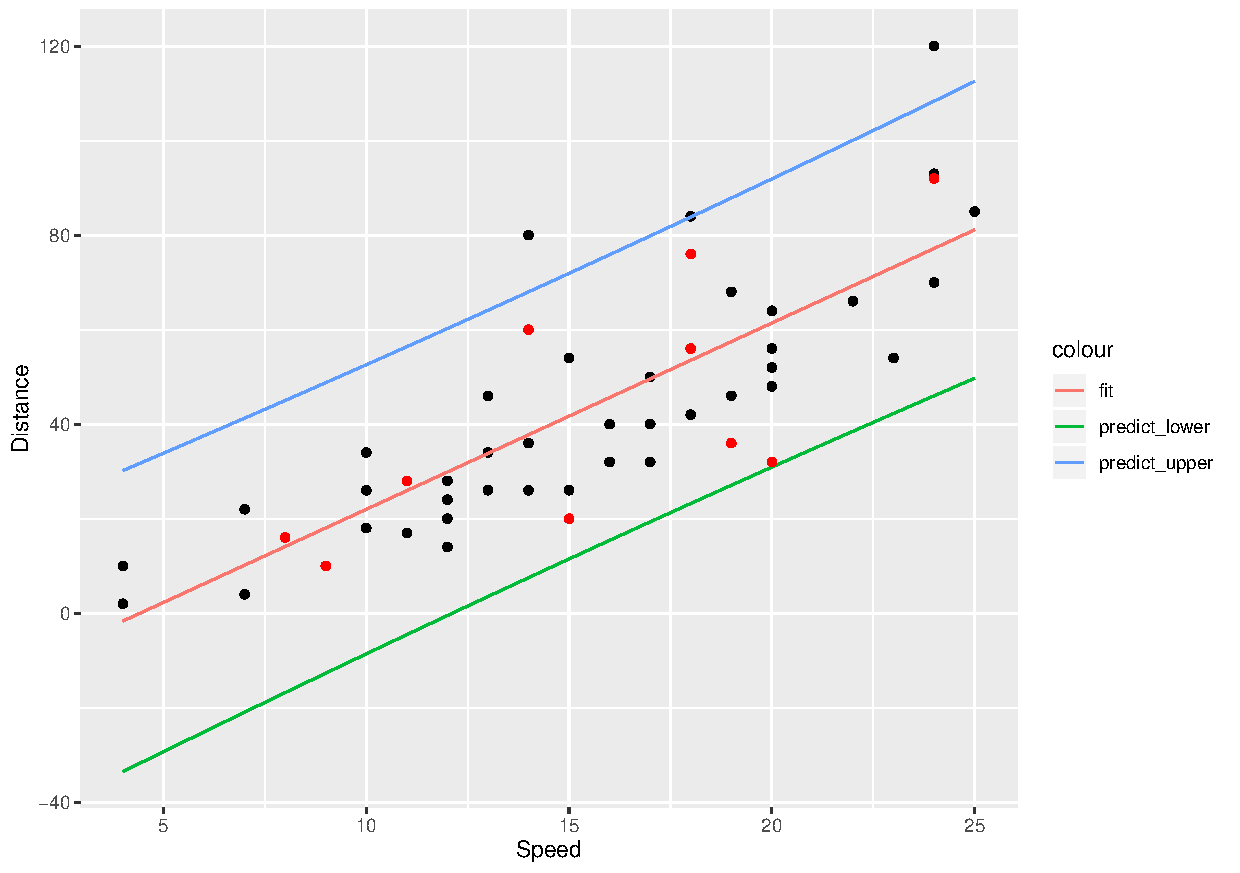
\includegraphics[width = 0.7\textwidth]{figures/Nanna/Prediction_plot.pdf}
    \caption{Plot of the observed values, the fitted regression line, its $95\%$-prediction intervals in which we expect new data points to be. The red data points are the new data points.}
    \label{fig:prediction}
\end{figure}



\end{example}


% \section{Confidence intervals}

% \begin{definition} [The (1-$\alpha$)-confidence Region]
% \label{def:confidence_region}
% Suppose that for a given number $\alpha \in (0,1)$ and for each $\textbf{y} \in \mathcal{Y}$, we have specified a subset $A(\textbf{y})$ of the parameter space $\Theta^k$, such that
% \begin{align*}
%     P_{\boldsymbol{\beta}} (\boldsymbol{\beta} \in A(\textbf{Y})) = 1 - a, \quad \forall \boldsymbol{\beta} \in \Theta^k
% \end{align*}
% Then we call $A(y)$ a $(1-\alpha)$-confidence region for $\boldsymbol{\beta}$.
% \end{definition}

% If the parameter is one-dimensional $(k=1)$ and the observations, $y$ are normally distributed, then the confidence region become the interval

% \begin{align*}
%     \left[ 
%     \hat{\beta}(\textbf{y}) + \Phi_{\alpha/2} \sqrt{D(\hat{\beta}(\textbf{y})} , \hat{\beta}(\textbf{y}) + \Phi_{1 - \alpha/2} \sqrt{D(\hat{\beta}(\textbf{y})}
%     \right]
% \end{align*}

% for $0 < \alpha \leq 0.5$. 


% \begin{example}
% Consider again the situation from example \ref{ex:model1}. By theorem \ref{th:distribution_ml_estimator} the asymptotic distribution of the ML estimator is given by
% \begin{align*}
%     \betahat \rightarrow^\mathcal{D} N\left( \mathbf{ \beta }, \boldsymbol{i}(\betahat)^{-1} \right)
% \end{align*}
% Since $\mathbf{\beta}$ is one-dimensional, $k=1$, and for $0\leq \alpha \leq 0.5$ we have the approximate $(1-\alpha)$-confidence interval
% \begin{align*}
% \left[ \betahat(\mathbf{y}) + \Phi_{\alpha/2} \sqrt{D\left( \betahat\left(\mathbf{y}\right)\right)}, \betahat(\mathbf{y}) + \Phi_{1 - \alpha/2} \sqrt{D\left( \betahat\left(\mathbf{y}\right)\right)} \right],
% \end{align*}
% where $D\left(\betahat(\mathbf{y})\right) = j\left(\betahat(\mathbf{y})\right)^{-1}$.
% For $\alpha=0.05$ we have the approximate $95\%$-confidence interval for $\mathbf{\beta}$:
% \begin{align*}
% \left[ \bar{y} - \frac{1.96}{\sqrt{n}}, \bar{y} + \frac{1.96}{\sqrt{n}} \right]    
% \end{align*}
% \end{example}

\section{F Test}
Suppose we want to test if a model has redundant explanatory variables.
In terms of hypothesis testing this is the null hypothesis: A set of variables has no statistically significant effect on $\textbf{y}$, once another set of variables has been controlled for.

Determining this will be done by analyzing the change in SSR, that is the difference in how well the models explain the data, and determining whether this change is significant. 
Suppose we have model 1 with $(k+1)$ variables 
\begin{align*}
    \textbf{y} = X \betabold +\  \varepsilon,
\end{align*}
this is known as the unrestricted model. The restricted model or model 0 lacks the $q$ variables, for which we want to check significance, that is
\begin{align*}
    \textbf{y} = \beta_0 + \beta_1 \textbf{x}_1 + \cdots + \beta_{k-q} \textbf{x}_{k-q} + \varepsilon.
\end{align*}
Therefore $q$ is the difference in df between the two models.
This means we want to test the hypothesis
\begin{align}
    \mathcal{H}_0: \beta_{k-q+1} = \ldots = \beta_k = 0.
\end{align}
These are referred to as the exclusion restrictions. 
This is done using the F statistic
\begin{align}\label{eq:F_statistic}
    F \equiv \frac{\| \textbf{H}_1 \textbf{y} - \textbf{H}_0 \textbf{y} \|^2/q}{\| \textbf{y} - \textbf{H}_1 \textbf{y} \|^2/(n-k-1)},
\end{align}
that is the relative increase in $SSR$, when going from model 0 to model 1. 
$\| \textbf{y} - \textbf{H}_0 \textbf{y} \|^2$ is the $SSR$ of model 0 and $\| \textbf{y} - \textbf{H}_1 \textbf{y} \|^2$ is that of model 1. 
$q$ is referred to as the numerator degrees of freedom, and $(n-k-1)$ is the denominator degrees of freedom. 

The change in SSR, when going from model 0 to model 1, is always non-negative because the model has more parameters to explain the data. 
This is discussed further in theorem \ref{th:Likelihood_ratio_linear_models}.

We will therefore reject $\mathcal{H}_0$, when $F$ is sufficiently large, since this indicates that significantly more of the variation of the data has been explained by model 1, as compared to model 0.

As with the t test, there is no correct significance level, but $\alpha = 5 \%$ is often chosen. 
The critical value for the significance level can be determined by calculating one explicitly from the cdf of the F distribution found below see definition \ref{def:F-distribution}. 
This is equivalent to the procedure for $t$-test.

$\mathcal{H}_0$ is therefore rejected if the F statistic is greater than the critical value
\begin{align*}
    F>c.
\end{align*}
If this is the case, the explanatory variables $\textbf{x}_{k-q+1}, \ldots, \textbf{x}_k$ are said to be jointly statistically significant. 
Otherwise they are said to be jointly insignificant, which can justify removing them from the model. 
In order to determine the critical value, the F distribution is given.
\begin{definition}[F Distribution]\label{def:F-distribution}
    Let $X_1 \sim \chi_{k_1}^2$ and $X_2 \sim \chi_{k_2}^2$ be independent random variables. Then the random variable 
        \begin{align*}
            F(k_1,k_2) = \frac{X_1/k_1}{X_2/k_2}
        \end{align*}
    has an F distribution with $(k_1, k_2)$ degrees of freedom, which is denoted as $F(k_1,k_2) \sim F_{k_1, k_2}$.
\end{definition}
The p-value for the F-test is analogouse to that of the t-test
\begin{align*}
    p = P(F(q,n-k-1) > F).
\end{align*}
That is the probability of observing this F-statistic under $H_0$. The confidence level therefore reflects how sure we are that the model under $H_0$ has generated the data.

\begin{example}
    As seen above we only need the degrees of freedom in order to find the F-distribution and thereby the critical value, for a given significance level.
    Firstly our data-set and models are introduced
    
    \begin{lstlisting}
        linreg1 <- lm(dist~speed,data=cars)
        linreg2 <- lm(dist~speed+I(speed^2),data=cars)
        n <- 50
        df1 <- n - 2
        df2 <- n - 3
    \end{lstlisting}
    
    The pdf for our F-distribution is then found using the 'df' function in R, not to be confused with the degrees of freedom. 
    
    \begin{lstlisting}
        dist_df <- data.frame(
        x = seq(0, 4, by = 0.01),
        pdf = df(x = seq(0, 4, 0.01), df1 = df1, df2 = df2)
        )
    \end{lstlisting}
    
    We choose a significance level of $a = 0.05$, from which we get the critical value $c=1.62$. This is found using the quantile function
    
    \begin{lstlisting}
        upper = qf(0.95, df1 = df1, df2 = df2)
    \end{lstlisting}
    
    The pdf and associated critical value are now plotted
    
    \begin{lstlisting}
        ggplot(aes(x = x, y = pdf), data = dist_df) + 
        geom_line() +
        #Highlighting the significans level
        geom_area(data=dist_df[which(dist_df$x > upper),],
        aes(x=x, y=pdf), fill = "red", alpha = 0.6)
    \end{lstlisting}
    
    \begin{figure}[H]
        \centering
      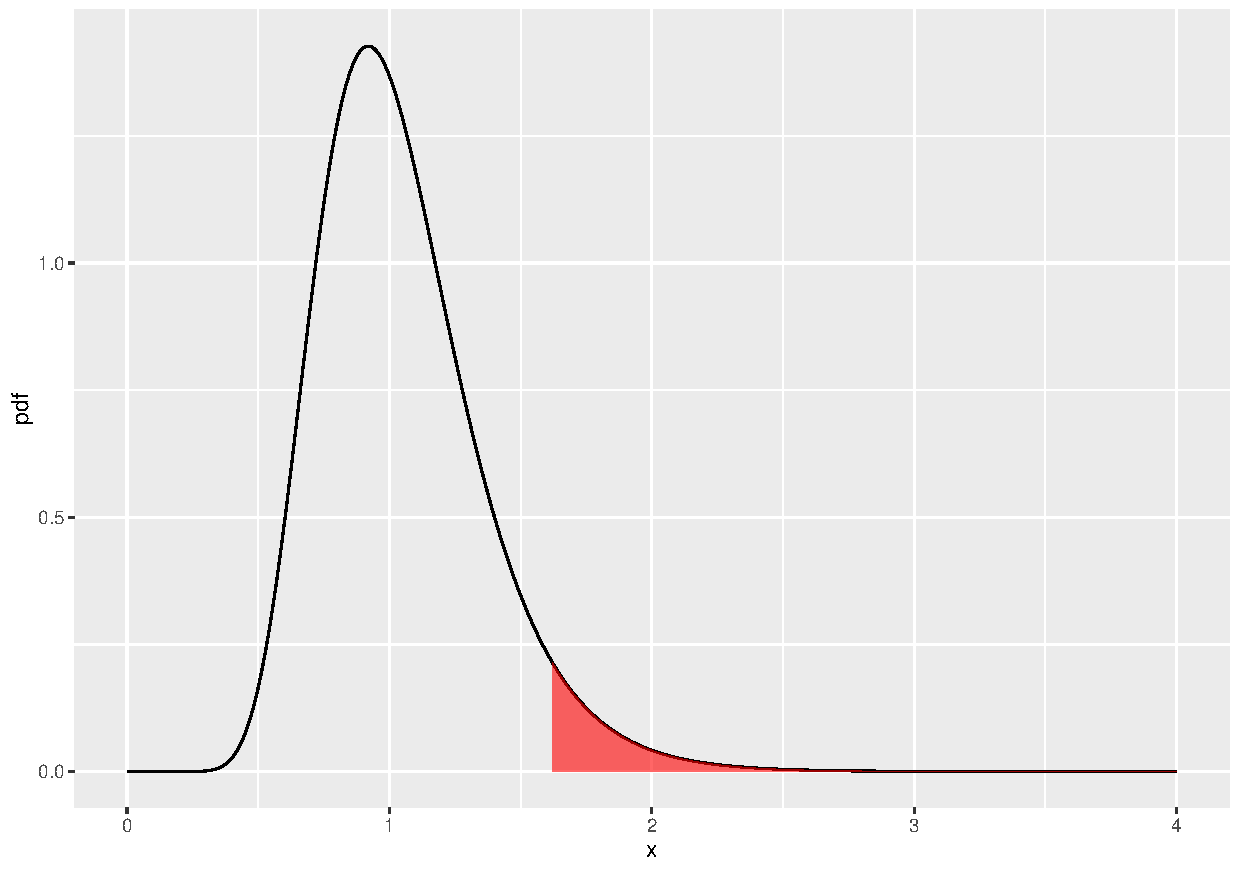
\includegraphics[width = 1 \textwidth]{figures/Thea/Fdistsign.pdf}
      \caption{Pdf for F-distribution with significance level}
      \label{fig:my_label}
    \end{figure}
    
    The significance level is illustrated by the area under the curve marked with red, and has the area equal to the significance level.
    
    The F-statistic is calculated using \eqref{eq:F_statistic}, where the SSR for the two models are calculated by the 'anova' function in R. 
    %Kode til Fstat
    \begin{lstlisting}
        RSS_model1 <- anova(linreg1,linreg2)$RSS[1]
        RSS_model2 <- anova(linreg1,linreg2)$RSS[2]
        Fstat <- ((RSS_model1 - RSS_model2)/(df1 - df2))/((RSS_model2)/df2)
        2.296027
    \end{lstlisting}
    
    The associated p-value is then
    
    \begin{lstlisting}
        p <- pf(q = Fstat, df1 = df1, df2 = df2, lower.tail=F)
        0.002517047
    \end{lstlisting}
    
    We conclude that the parameter $speed^2$ is with 95\% certainty statistically significant.
\end{example}

The likelihood ratio can compare the goodness of fit for 2 models, specifically one over the entire parameter space and one with a restriction imposed.
It would therefore be interesting to see what relation it has to the F-test.

\begin{theorem}[Likelihood Ratio For Linear Models]
\label{th:Likelihood_ratio_linear_models}
    The Likelihood ratio
    \begin{align*}
        \lambda(y) = \frac{\sup \ L(\mu_0, \sigma_0^2; y)}{\sup \ L(\mu_1, \sigma_1^2; y)}
    \end{align*}
    is a strictly decreasing function of $F(y)$ under $\mathcal{H}_0$, such that
    \begin{align*}
        F(Y) \sim F(q, n-k-1).
    \end{align*}
\end{theorem}

\begin{proof}
    Under $\mathcal{H}_1$: $\hat{\mu}_1 = H_1 y$ and $\hat{\sigma}_1^2 = \frac{\| y - H_1 y \|^2}{n}$, the log likelihood function is
    \begin{align*}
        l(\hat{\mu}_1, \hat{\sigma}_1^2; y) &= -\frac{n}{2} log(\hat{\sigma}_1^2) - \frac{1}{2 \hat{\sigma}_1^2} \| y - H_1 y \|^2 \\
        &= -\frac{n}{2} log(\hat{\sigma}_1^2) - \frac{n}{2},
    \end{align*}
    and similarly for $\mathcal{H}_0$. Therefore the likelihood ratio can be written as
    \begin{align*}
        \lambda(y) &= exp \left( l(\hat{\mu}_0, \hat{\sigma}_0^2; y) - l(\hat{\mu}_1, \hat{\sigma}_1^2; y) \right) \\
        &= exp \left( -\frac{n}{2} \Big( log(\hat{\sigma}_0^2) - log(\hat{\sigma}_1^2)\Big) \right) \\
        &= \left( \frac{\| y - H_1 y \|^2}{\| y - H_0 y \|^2} \right)^{\frac{n}{2}} \\
        &= \left( \frac{\| y - H_1 y \|^2}{\| y - H_1 y \|^2 + \| H_1 y - H_0 y \|^2} \right)^{\frac{n}{2}}.
    \end{align*}
    The last equation holds because $y - H_1 y$ is orthogonal to $\Omega_1$ and $(H_1 y - H_0 y) \in \Omega_1$. Dividing by the numerator and using \eqref{eq:F_statistic}, the above equation becomes
    \begin{align*}
        \lambda(y) &= \left( \frac{1}{1 + \frac{\| H_1 y - H_0 y \|^2}{\| y - H_1 y \|^2}} \right)^{\frac{n}{2}} \\
        &= \left( \frac{1}{1 + \frac{q}{n-k-1}F(y)}  \right)^{\frac{n}{2}}.
    \end{align*}
    The likelihood ratio is therefore a function of $F$, and since it is in the denominator, $\lambda(y)$ is a decreasing function of $F(y)$. We again see that large values of $F$ are critical, since small values of $\lambda(y)$ are critical.
    
    The fact that $F$ is F-distributed is seen from
    \begin{align*}
        F(Y) &= \frac{\| H_1 Y - H_0 Y \|^2/q}{\| Y - H_1 Y \|^2/(n-k-1)} \\
        &= \frac{\| (H_1 - H_0) Y \|^2/q}{\| (I - H_1) Y \|^2/(n-k-1)} \\
        &\sim \frac{\chi^2(q)/q}{\chi^2(n-k-1)/(n-k-1)}, \\
    \end{align*}
    cf. definition \ref{def:F-distribution}. Here the last equation holds because $H_1 - H_0$ and $I - H_1$ are projections, and therefore follow a chi-squared distribution.
\end{proof}

\begin{theorem}
    The $t$-test in \eqref{eq:t-test} is equivalent to the likelihood ratio test for $\mathcal{H}_0 \ : \ \beta_j = \beta_{0j}$.
\end{theorem}
\begin{proof}
    Without loss of generality assume that $j = 1$.
    Let $\betabold_{-1} = (\beta_2, \ldots, \beta_k)^\top$, so $\betabold = (\beta_1, \beta_{-1}^\top)^\top$.
    Denote by $\textbf{x}_1$, the first column of $\textbf{X}$, and by $\textbf{X}_{-1}$, the remaining columns of $\textbf{X}$, such that $\textbf{X} = \left[\textbf{x}_1 \ \textbf{X}_{-1}\right]$.
    
    Consider first the case $\beta_{01} = 0$: Then $\textbf{X}_{-1}$ is the design matrix for $\mathcal{H}_0$.
    The hat matrices corresponding to $\textbf{X}$ and $\textbf{X}_{-1}$ are given by
    \begin{align*}
        \textbf{H} = \textbf{X}(\textbf{X}^\top\textbf{X})^{-1}\textbf{X}^\top, \quad \mathbf{H}_{-1} = \textbf{X}_{-1}(\textbf{X}^\top_{-1}\textbf{X}_{-1})^{-1}\textbf{X}^\top_{-1},
    \end{align*}
    respectively.
    The MLE for the mean vector under the original model is $\textbf{H}\textbf{y}$, the MLE for the mean vector under $\mathcal{H}_0$ is $\textbf{H}_{-1}\textbf{y}$, and the $F$-statistic for $\mathcal{H}_0$ is
    \begin{align*}
        F(\textbf{y}) = \frac{\|\textbf{H}\textbf{y} - \textbf{H}_{-1}\textbf{y}\|^2/(k-(k-1))}{\hat{\sigma}^2(\textbf{y})}
    \end{align*}
    where large values of $F(\textbf{y})$ are critical for $\mathcal{H}_0$.
    We have
    \begin{align*}
        \textbf{H}\textbf{y} = \textbf{X}\betahat(\textbf{y}) = \textbf{x}_1\hat{\beta}_1(\textbf{y}) + \textbf{X}_{-1} \betahat_{-1}(\textbf{y})
    \end{align*}
    and $\textbf{H}_{-1}\textbf{H} = \textbf{H}_{-1}$, so
    \begin{align*}
        \textbf{H}\textbf{y}-\textbf{H}_{-1}\textbf{y} = 
        \textbf{H}\textbf{y}-\textbf{H}_{-1}\textbf{H}\textbf{y} =
        (\textbf{I} - \textbf{H}_{-1})\textbf{H}\textbf{y} = 
        (\textbf{I} - \textbf{H}_{-1})\textbf{x}_1\hat{\beta}_1(\textbf{y})
    \end{align*}
    since $(\textbf{I} - \textbf{H}_{-1})\textbf{X}_{-1} = 0$.
    Hence, as $\textbf{I} - \textbf{H}_{-1}$ is symmetric and idempotent,
    \begin{align*}
        \|\textbf{H}\textbf{y} - \textbf{H}_{-1}\textbf{y}\|^2 = \hat{\beta}_1(\textbf{y})^2\textbf{x}_1^\top(\textbf{I} - \textbf{H}_{-1})\textbf{x}_1.
    \end{align*}
    In appendix \ref{ch:block_matrix_inversion} it is verified that $\textbf{x}_1^\top(\textbf{I} - \textbf{H}_{-1})\textbf{x}_1 = 1/d_1$.
    Consequently,
    \begin{align*}
        F(\textbf{y}) = \frac{\hat{\beta}(\textbf{y})^2/d_1}{\hat{\sigma}^2(\textbf{y})} = t_1(\textbf{y};0)^2
    \end{align*}
    and so the $t$-test in theorem (specify which) is equivalent to the $F$-test which in turn is equivalent to the likelihood ratio test.
    
    Consider next the general case where $\beta_{01}$ is any fixed number: Let $\textbf{Z} = \textbf{Y} - \textbf{x}_1\beta_{01}$ and
    \begin{align*}
        \Tilde{\betabold} = (\beta_1 - \beta_{01}, \beta_2, \ldots, \beta_k)^\top = \betabold - (\beta_{01}, 0, \ldots, 0)^\top.
    \end{align*}
    Since $\textbf{Z} \sim N_n(\textbf{X}\Tilde{\boldsymbol{\beta}}, \sigma^2\textbf{I}_n)$ and $\{ (\beta_1 - \beta_{01}, \beta_2, \ldots, \beta_k)^\top \ : \ \beta_1 \in \mathbb{R}, \ldots, \beta_k \in \mathbb{R} \} = \mathbb{R}^k$, we see that $\textbf{Z}$ corresponds to $\textbf{Y}$ in the first case.
    It is easily seen that
    \begin{align*}
        \hat{\boldsymbol{\sigma}}^2(\textbf{Z}) = \hat{\boldsymbol{\sigma}}^2(\textbf{Y}), \quad \hat{\bar{\boldsymbol{\beta}}}(\textbf{Z}) = \hat{\boldsymbol{\beta}}(\textbf{Y}) - (\beta_{01}, 0, \ldots, 0)^\top,
    \end{align*}
    since the MLE is invariant under reparametrizations and under one-to-one transformations of the data.
    Combining these facts we obtain
    \begin{align*}
        F(\textbf{z}) =
        \frac{\hat{\bar{\boldsymbol{\beta}}}(\textbf{Z})^2/d_1}{\hat{\boldsymbol{\sigma}}^2(\textbf{z})} = 
        \frac{(\betahat(\textbf{y}) - \beta_{01})^2/d_1}{\hat{\boldsymbol{\sigma}}^2(\textbf{y})}
    \end{align*}
    which completes the proof.
\end{proof}

In practice it can be useful to express the F-statistic as a function of $R^2$ instead of $SSR$, as it can become large, making computation slower, whereas $R^2$ is always between $0$ and $1$. In addition many programs often report $R^2$ and not $SSR$.

This form of the F statistic is obtained by using the equality's $SSR_0 = SST(1 - R^2_0)$ and $SSR_1 = SST(1-R^2_1)$. Substituting these into \eqref{eq:F_statistic} yields
\begin{align}\label{eq:F_test_R}
    F &= \frac{(SST(1 - R^2_0) - SST(1-R^2_1)/q}{SST(1-R^2_1)/(n-k-1)} \nonumber \\
    F &= \frac{(R^2_1 - R^2_0)/q}{(1 - R^2_1)/(n-k-1)}.
\end{align}

In addition the F-statistics can be used to test for the overall significance of a regression. Consider the model with $k$ independent variables, to which the null hypothesis can be written as
\begin{align}\label{eq:null_hypo_for_F_overall_significance_R}
    \mathcal{H}_0: \betabold_1 = \betabold_2 = \ldots = \betabold_k = 0.
\end{align}
Where the alternative hypothesis is that at least one estimator is non-zero. In \eqref{eq:null_hypo_for_F_overall_significance_R} there are $k$ restrictions and they state that knowing the values of the explanatory variables does not explain the dependent variable $y$. This can be written as
\begin{align}\label{eq:unrestricted_F_hypo_for_jeg_skal_bruge_den}
    y = \betabold_0 + \ \varepsilon
\end{align}
Where all independent variables have been excluded due to no affect on $y$. 
Recall equation \eqref{eq:F_test_R}, which is the F-statistics using the $\mathcal{R}$-squared. 
In the restricted model \eqref{eq:unrestricted_F_hypo_for_jeg_skal_bruge_den} the $\mathcal{R}$-squared is equal to $0$ because none of the variation in $y$ is accounted for because there are no explanatory variables. 
Furthermore $q = df_0 - df_{1}$ is equal to $k$ because $df_0 = n-0-1$ and $df_{1} = n-k-1$ which means $q = n-1 - (n-k-1) = k$. If we substitute this into \eqref{eq:F_test_R} we get
\begin{align}\label{eq:udvidelse_til_F_stat}
    F = \dfrac{\mathcal{R}^2_{\hat{\varepsilon}^2}/k}{(1-\mathcal{R}^2_{\hat{\varepsilon}^2}) / (n-k-1)}
\end{align}
This F-statistics in only valid in testing for joint exclusion of all independent variables. 
Therefore it often referred to as the overall significance of the regression. 

\subsection{Test for Heteroscedasticity}
In this section we wish to introduce a method to determine if heteroskedasticity is present, because in the case of heteroskedasticity the usual OLS estimator is not BLUE. 

We consider our linear model given as $y = \mathbf{\beta}_0 + \mathbf{\beta}_1x_1 + \ldots + \mathbf{\beta}_kx_k + \mathbf{\varepsilon}$ and let assumption \ref{as:linear_in_the_parameters}, \ref{as:no_perfect_collinearity} and \ref{as:zero_conditional_mean} hold.

We then construct our null hypothesis as
\begin{align*}
    \mathcal{H}_0 : \var[\varepsilon | \mathbf{X}] = \var[\varepsilon] = \sigma^2. 
\end{align*}
With this null hypothesis we wish to determine if the homoskedasticity assumption holds. 
If we accept our $\mathcal{H}_0$-hypothesis for a small significance level then heteroskedasticity is with a high probability not present.
Assumption \ref{as:zero_conditional_mean}, which says that the conditional expected value is equal to $0$, implying that $\var(\varepsilon | \mathbf{X}) = E[\varepsilon^2 | \mathbf{X}]$ because of the conditional variance formula $\var(\varepsilon | \mathbf{X}) = E[\varepsilon^2 | \mathbf{X}] - (E[\varepsilon | \mathbf{X}])^2$. Using this we rewrite our $\mathcal{H}_0$-hypothesis as
\begin{align*}
    \mathcal{H}_0 : E[\varepsilon^2 | \mathbf{X}] = E[\varepsilon^2] = \sigma^2.
\end{align*}
With this $\mathcal{H}_0$-hypothesis we test if the error term, $\sigma^2$ is related with any of the explanatory variables in terms of the expected value.  
If $\mathcal{H}_0$ is rejected then $\varepsilon^2$ is a function of at least one of the explanatory variables, so the error term can be expressed as a linear function of these explanatory variables
\begin{align}\label{eq:test_hetero_nul_hypotese}
    \varepsilon^2 = \delta_0 + \delta_1x_1 + \ldots + \delta_kx_k + v
\end{align}
Where $v$ is an error with mean equal to $0$ given the explanatory variables. In order for $\varepsilon^2$ to be homoskedastic the following $\mathcal{H}_0$-hypothesis must be accepted 
\begin{align}\label{eq:H_nul_for_hetero_med_delta}
    \mathcal{H}_0 : \delta_1 = \delta_2 = \ldots = \delta_k = 0
\end{align}
So the error term $v$ does not depend on the explanatory variables. If the error $v$ in \eqref{eq:test_hetero_nul_hypotese} is assumed to be independent of the explanatory variables $\mathbf{X}$, then F-statistics can be used to test \eqref{eq:H_nul_for_hetero_med_delta} for the overall significance of the explanatory variables for $\varepsilon^2$, even though this error term is not normally distributed. We state the central limit theorem without proof to justify this. 
\begin{theorem}[Central Limit Theorem] \label{th:Central_limit_theorem}
Let $\{ Y_1, Y_2, \ldots, Y_n \}$ be a iid. random sample with mean $\mu$ and variance $\sigma^2 < \infty$. Then
\begin{align*}
    P\left(\dfrac{\overline{Y}_n - n\mu}{\sigma \sqrt{n}}\leq y\right) \rightarrow \Phi(y)
\end{align*}
Where $\Phi(y)$ is the cdf of the standard normal distribution. 
\end{theorem}
From the central limit theorem it is possible to derive the distribution of $\overline{Y}_n$. We have  
\begin{align*}
    P\left(\dfrac{\overline{Y}_n - n\mu}{\sigma \sqrt{n}} \leq y\right) \rightarrow \Phi(y)
\end{align*}
And for large $n$ we use the central limit theorem to rewrite as
\begin{align*}
    Z_n = \dfrac{\overline{Y}_n - n\mu}{\sigma \sqrt{n}} \stackrel{d}{\approx} N(0,1). 
\end{align*}
Where $\stackrel{d}{\approx}$ denotes the approximate distribution. It is seen that $\overline{Y}_n$ has mean $n\mu$ and variance $n \sigma^2$ from the above equation. We use this to write
\begin{align*}
    \overline{Y}_n \stackrel{d}{\approx} N(n\mu, n\sigma^2). 
\end{align*}
This means that iid. random variables have an approximate normal distribution regardless of the distribution of $Y$. It then follows that an F-statistic will be asymptotically true even though $\varepsilon^2$ is not normally distributed. 

Since $\varepsilon^2$ is unobserved we cannot calculate the OLS regression on $\varepsilon^2$ for $\mathbf{X}$, so instead we calculate the regressions using the estimates. Thus
\begin{align}\label{eq:OLS_residual_hat_epsioln_i_anden}
    \hat{\varepsilon}^2 = \delta_0 + \delta_1x_1 + \ldots + \delta_kx_k + w
\end{align}
Where $\hat{\varepsilon}_i$ is an estimate for $\varepsilon_i$ for observation $i$. From this equation the F-statistics for the joint significance of $x_1, x_2, \ldots, x_k$ can be calculated to test for multicollinarity. 

The F-statistics is calculated as
\begin{align*}
    F = \dfrac{\mathcal{R}^2_{\hat{\varepsilon}^2}/k}{(1-\mathcal{R}^2_{\hat{\varepsilon}^2}) / (n-k-1)}
\end{align*}

Which follows from \eqref{eq:udvidelse_til_F_stat}. Here $\mathcal{R}^2_{\hat{\varepsilon}^2}$ is the $\mathcal{R}$-squared found from \eqref{eq:OLS_residual_hat_epsioln_i_anden} and $k$ is the number of independent variables in \eqref{eq:OLS_residual_hat_epsioln_i_anden}. 

This procedure is known as the \textbf{Breush-Pegan Test for heteroskedasticity}. We summarise the steps as follows

\textbf{The Breusch-Pegan Test for Heteroskedasticity}
\begin{enumerate}[label=(\roman*)]
    \item Estimate the linear regression model \eqref{eq:multiple_linear_regression_model} by OLS and obtain the squared OLS residuals $\hat{\varepsilon}^2$. 
    \item Make the regression on \eqref{eq:OLS_residual_hat_epsioln_i_anden} and calculate the $\mathcal{R}^2_{\hat{\varepsilon}^2}$. 
    \item Perform the F-statistics. If the p-value is below the significance level, reject the null hypothesis. 
\end{enumerate}

This means that if the p-value if sufficiently small for the F-statistics, then heteroskedasticity is present. 

\begin{example}[Test for Heteroskedasticity]

\end{example}

\subsection{Type of Heteroskedasticity}
In addition to testing for the presence of heteroskedasticity, it is possible to test for the type of heteroskedasticity. 



\subsection{Correct for Heteroscedasticity}
To sum up \hetero will in general cause OLS standard errors to be faulty as well as the related statistical tests. In this section we wish to correct for these mistakes, so they are correct when \hetero is present.




















\section{Residuals}\label{subsec:residuals}

The residuals are the difference between the observed values $y$ and the fitted values $\hat{y}$. They are therefore the errors $\boldsymbol{\hat{\varepsilon}}$ described in \eqref{eq:replace_with_y}
\begin{align*}
    r(\textbf{y}) &= \textbf{y} - \hat{\textbf{y}} = \textbf{y} - \textbf{X} \betahat = (I - H) \textbf{y}.
    % r_i(y) &= y_i - x_i \betahat = y_i - x_i (X^\top X)^{-1}X^\top y_i = (1 - h_{ii}) y_i,
\end{align*}
By assumption \ref{as:normality_of_errors} the residuals have variance
\begin{align*}
    Var(r(\textbf{Y})) &= \sigma^2 (I - H) \\
    Var(r_i(\textbf{Y})) &= \sigma^2(1 - h_{ii}),
\end{align*}
where $h_{ii}$ is the i'th diagonal element in $H$. The second equation follows, since the first equation is just the variance-covariance matrix for the residuals, which has variances in the diagonal.
Rewriting \eqref{eq:sigma_hat_2_n-k-1} using projection matrices gives the following estimate for the parameter variance
\begin{align*}
    \hat{\sigma}^2(\textbf{Y}) &= \frac{\| \textbf{Y} - \textbf{X} \betahat (\textbf{y}) \|^2 }{n-k-1} = \frac{\| \textbf{Y} - \textbf{H} Y \|^2}{n-k-1} .
\end{align*}
Residuals can be used to identifiy outliers, which is the observations that do not fit the general pattern of the data.
These datapoints can have a large effect on the estimated variance and it would therefore be useful to have a way to measure of how much variance an observation adds.
We now introduce the notation $-i$, which refers to the removal of the i'th row e.g.
\begin{align*}
    \textbf{y}_{-i}^\top = (y_1, \ldots, y_{i-1}, y_{i+1}, \ldots, y_n)^\top.
\end{align*}
The estimate for $\sigma^2$ found by deleting the i'th row is then
\begin{align*}
    \hat{\sigma}^2_{(i)}(\textbf{Y}) = \frac{\| \textbf{Y}_{-i} - H_{-i} \textbf{Y}_{-i} \|^2}{n-k-1}.
\end{align*}
We now introduce the studentized residual $(r^{rt})$, which takes into account the variance without the i'th observation, thereby giving a more accurate measure of the standard deviation. 
\begin{align*}
    r_i^{rt} = \frac{r_i}{\sqrt{\hat{\sigma^2_{(i)}}(1-h_{ii})}}.
\end{align*}
If this value in deemed to high, it should be investigated and could potentially justify removing it as an outlier/measurement error. We now introduce an important property of the studetized residuals.

\begin{proposition}
    Consider a general linear model $Y \sim N_n(X \betahat, \sigma^2 I_n)$ where the design matrix has full rank $k \leq n-3$ and $H = X (X^\top X)^{-1}X^\top$ is the corresponding projection-matrix, then
    \begin{align*}
        r_i^{rt}(\textbf{Y}) \sim t(n-k-1).
    \end{align*}
\end{proposition}
\begin{proof}
    Without loss of generality let $i=1$. 
    To summarize the above results
    \begin{align*}
        r_i^{rt} = \frac{r_1}{\sqrt{\hat{\sigma^2_{(1)}}(1-h_{11})}}
        =
        \frac{r_1(Y)/ \sqrt{\sigma^2 (I-h_{11})}}{\sqrt{\hat{\sigma}_1^2 (Y_{-1})/\sigma^2}},
    \end{align*}
    which has the distribution
    \begin{align*}
        \frac{N(0,1)}{\sqrt{\chi^2(n-k-1)/(n-k-1)}} = t(n-k-1)
    \end{align*}
    Therefore we just need to prove that they are independent.
    Using the definition of the residual and the projection matrix
    \begin{align*}
        \begin{bmatrix}
            r_1(\textbf{Y}) \\
            \textbf{Y}_{-1} - H_{-1} \textbf{Y}_{-1}
        \end{bmatrix}
        =
        \begin{bmatrix}
            Y_1 - \textbf{x}_1^\top (\textbf{X}^\top \textbf{X})^{-1} X^\top \textbf{Y} \\
            \textbf{Y}_{-1} - \textbf{X}_{-1} (\textbf{X}_{-1}^\top \textbf{X}_{-1})^{-1} \textbf{X}_{-1}^\top \textbf{Y}_{-1}
        \end{bmatrix}
    \end{align*}
    This can be written as the matrix-vector product
    \begin{align*}
        \begin{bmatrix}
            1 - \textbf{x}_1^\top (\textbf{X}^\top \textbf{X})^{-1} \textbf{x}_1^\top & - \textbf{x}_1^\top (\textbf{X}^\top \textbf{X})^{-1} \textbf{X}_{-1}^\top \\
            0 & I_{n-1} - \textbf{X}_{-1} (\textbf{X}_{-1}^\top \textbf{X}_{-1})^{-1} \textbf{X}_{-1}^\top
        \end{bmatrix}
        \begin{bmatrix}
            Y_1 \\
            \textbf{Y}_{-1}
        \end{bmatrix}
        =
        AY \sim N(\cdot)
    \end{align*}
    Therefore $r_1(Y) = AY$ and $A_2 = \textbf{Y}_{-1} - H_{-1} \textbf{Y}_{-1}$ are independent if they are uncorrelated. Their covariance matrix is given by 
    \begin{align*}
        cov(A Y, A_2 Y) &= A\  var(Y) \ A_2^\top = A \sigma^2 I A_2 = \sigma^2 A A_2 \\
        &= \sigma^2 
        \begin{bmatrix}
            1 - \textbf{x}_1^\top (\textbf{X}^\top \textbf{X})^{-1} \textbf{x}_1^\top & - \textbf{x}_1^\top (\textbf{X}^\top \textbf{X})^{-1} \textbf{X}_{-1}^\top
        \end{bmatrix}
        \cdot
        \begin{bmatrix}
            0^\top \\
            I_{n-1} - \textbf{X}_{-1} (\textbf{X}_{-1}^\top \textbf{X}_{-1})^{-1} \textbf{X}_{-1}^\top
        \end{bmatrix} \\
        &= \sigma^2 (- \textbf{x}_1^\top (\textbf{X}^\top \textbf{X})^{-1} \textbf{X}_{-1}^\top) (I_{n-1} - \textbf{X}_{-1} (\textbf{X}_{-1}^\top \textbf{X}_{-1})^{-1} \textbf{X}_{-1}^\top) \\
        &= \sigma^2 (- \textbf{x}_1^\top (\textbf{X}^\top \textbf{X})^{-1} \textbf{X}_{-1}^\top + \textbf{x}_1^\top (\textbf{X}^\top \textbf{X})^{-1} \textbf{X}_{-1}^\top \textbf{X}_{-1} (\textbf{X}_{-1}^\top \textbf{X}_{-1})^{-1} \textbf{X}_{-1}^\top)) \\
        &= \sigma^2 (- \textbf{x}_1^\top (\textbf{X}^\top \textbf{X})^{-1} \textbf{X}_{-1}^\top + \textbf{x}_1^\top (\textbf{X}^\top \textbf{X})^{-1} \textbf{X}_{-1}^\top)) \\
        &= 0,
    \end{align*}
    and therefore uncorrelated and because they are normally distributed also independant.
\end{proof}

Overall significance of the regression

TILFØJ SÆTNING SOM SAMMENLIGNER T TEST OG LIKELIHOOD RATION





